\documentclass[UTF8]{ctexart}
\usepackage{graphicx}
\usepackage{amsmath}
\title{基于数据并行化SVM阅读笔记}
\author{王忆麟}
\date{\today}
\begin{document}
\maketitle
\section{Cascade-SVM}
\subsection{算法简介}
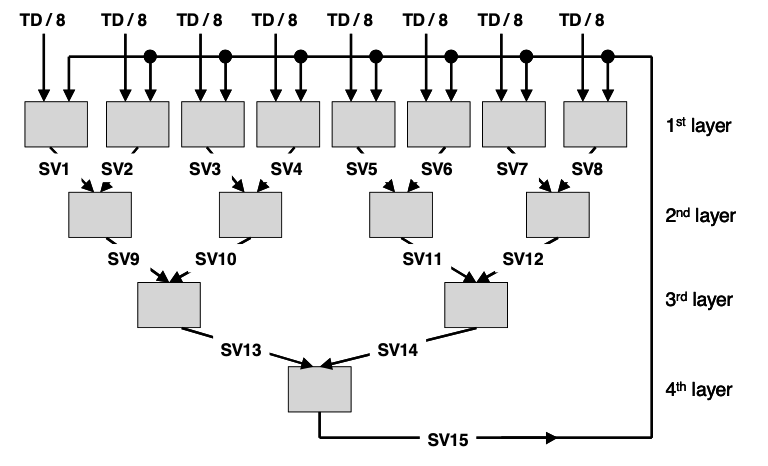
\includegraphics{cascade-svm.png}
\paragraph{
    Cascade-SVM是较早发表的一篇文章,算法思路并不复杂。
    首先,将原始训练集分发到各个计算节点上,在各个节点上分别训练svm,并两两合并,将支持向量合并到一起,并再进行svm训练,直至最后支持向量合并到同一节点。如果对结果不满意,还可以将最后一层上训练的支持向量再分发到所有节点上再训练,重复以上的过程,直至达到满意的效果。
}
\subsection{算法优缺点分析}
\paragraph{
    Cascade-SVM算法的优势在于,在最终计算前,先对各个节点上的数据进行训练,得到支持向量。再进行聚合,这样只需传递支持向量即可。但是这样仍然会造成较大的通信开销。因为最终仍需要将支持向量聚集到一个计算节点上。
}
\section{DC-SVM}
\subsection{算法分析}
\paragraph{
    DC-SVM是一种与Cascade-SVM相似的算法,但是我觉得DC-SVM的思路更值得借鉴,启发性更大。DC-SVM首先对数据进行k-means聚类(实际上由于kmeans聚类消耗的时间太多,改用了简化方法),再进行SVM训练。每次训练前,都从之前训练的支持向量中挑选出m(m为计算节点数)个初始的聚类中心,并进行聚类,再将对应的各个类发送到各个计算节点训练出SVM。每次训练完后,减少一半的训练节点,直至只有一个节点
}
\subsection{算法优缺点分析}
\paragraph{
    其实从算法描述来看,DC-SVM与Cascade-SVM十分相似,但是DC-SVM中有一个思路对我有一些启发。DC-SVM先提出了一个假设:设$\bar{\alpha}$是对偶问题在用$\bar{K}(x_i,x_j)=I(\pi(x_i),\pi(x_j))K(x_i,x_j))$函数替换$K(x_si,x_j)$情况下的最优解。其中$\pi(x_i)$是$x_i$所属的类别,$I(a,b)$在ab相同时为1,不同时为0。之后他们证明了
}
\[0 \leq f(\bar{\alpha})-f(\alpha^*) \leq \frac{1}{2}C^2D(\pi)\]
\paragraph{
    也就是说,如果将训练数据切成多块进行训练,得到的解和最优解之间的偏差是有上界的。我觉得这个思路可以为优化分布式SVM提供一个想法,可以考虑尽可能减小$D(\pi)$的值,直接在集群中分别训练,而不需要进行聚合操作,从而大大减小通信代价。
}

\end{document}
